% ========================================
% CHAPTER 5: EXPERIMENTS AND EVALUATION (ACTUAL SETUPS AND RESULTS)
% ========================================
\chapter{Experiments and Evaluation}

% ========================================
% SECTION 5.0: EXPERIMENTAL SETUP
% ========================================
\section{Experimental Setup}

We implement our ICAE framework from scratch, building upon the original architecture \cite{ge_-context_2024} with several modifications for improved efficiency and reproducibility. Our implementation uses Qwen3-8B as the base model, with LoRA adaptation applied to the attention matrices (q\_proj and v\_proj) using a rank of 128.

Pretraining is conducted on the SlimPajama-6B dataset using a combination of autoencoding and language modeling objectives, achieving 95\% reconstruction BLEU score on general text. Fine-tuning on SWE-bench trajectories uses a larger memory size of 256 tokens and explicitly disables thinking mechanisms for simplicity, focusing on direct tool-call generation.

Training was performed on a single NVIDIA H200 GPU, requiring approximately 1 day and 15 hours for pretraining and 3 days for fine-tuning due to the computational complexity of the autoencoding objective and resulting lack of effective batching opportunities.

Detailed hyperparameters and training configurations are provided in Appendix~\ref{app:training_details}.


% ========================================
% SECTION 5.1: INITIAL PROTOTYPE EXPERIMENTS: THE NECESSITY OF TRAINING
% ========================================
\section{Initial Prototype Experiments: The Necessity of Training}

The initial approach tested replacing hard tokens with soft/averaged continuous embeddings without fine-tuning.
These prototype experiments, using methods like KV-cache hacks or direct embedding inputs in vLLM, demonstrated that scores decreased by more than 50\% on QA tasks (e.g., SQuAD context embed F1 dropped from 0.71 to 0.17 or 0.11).
This negative result confirmed the hypothesis that training is necessary to effectively condense context into the latent space.

\begin{table}[h]
    \centering
    \begin{tabular}{lcc}
        \toprule
        \textbf{Setting (SQuAD), context embed} &
        \textbf{Exact Match} & \textbf{F1} \\
        \midrule
        Baseline — hard tokens         & \textbf{0.58} & \textbf{0.71} \\
        Hard embedded, avg ×2          & 0.09 & 0.21 \\
        Soft embedded online, avg ×2          & 0.05 & 0.11 \\
        Soft embedded \text{regenerate-llm} avg ×2          & 0.07 & 0.16 \\
        \bottomrule
    \end{tabular}
    \caption{Baseline against averaging techniques (Prompt–Q–C)}
    \label{tab:avg_variants}
\end{table}

\begin{figure}[hbt]
  \centering
  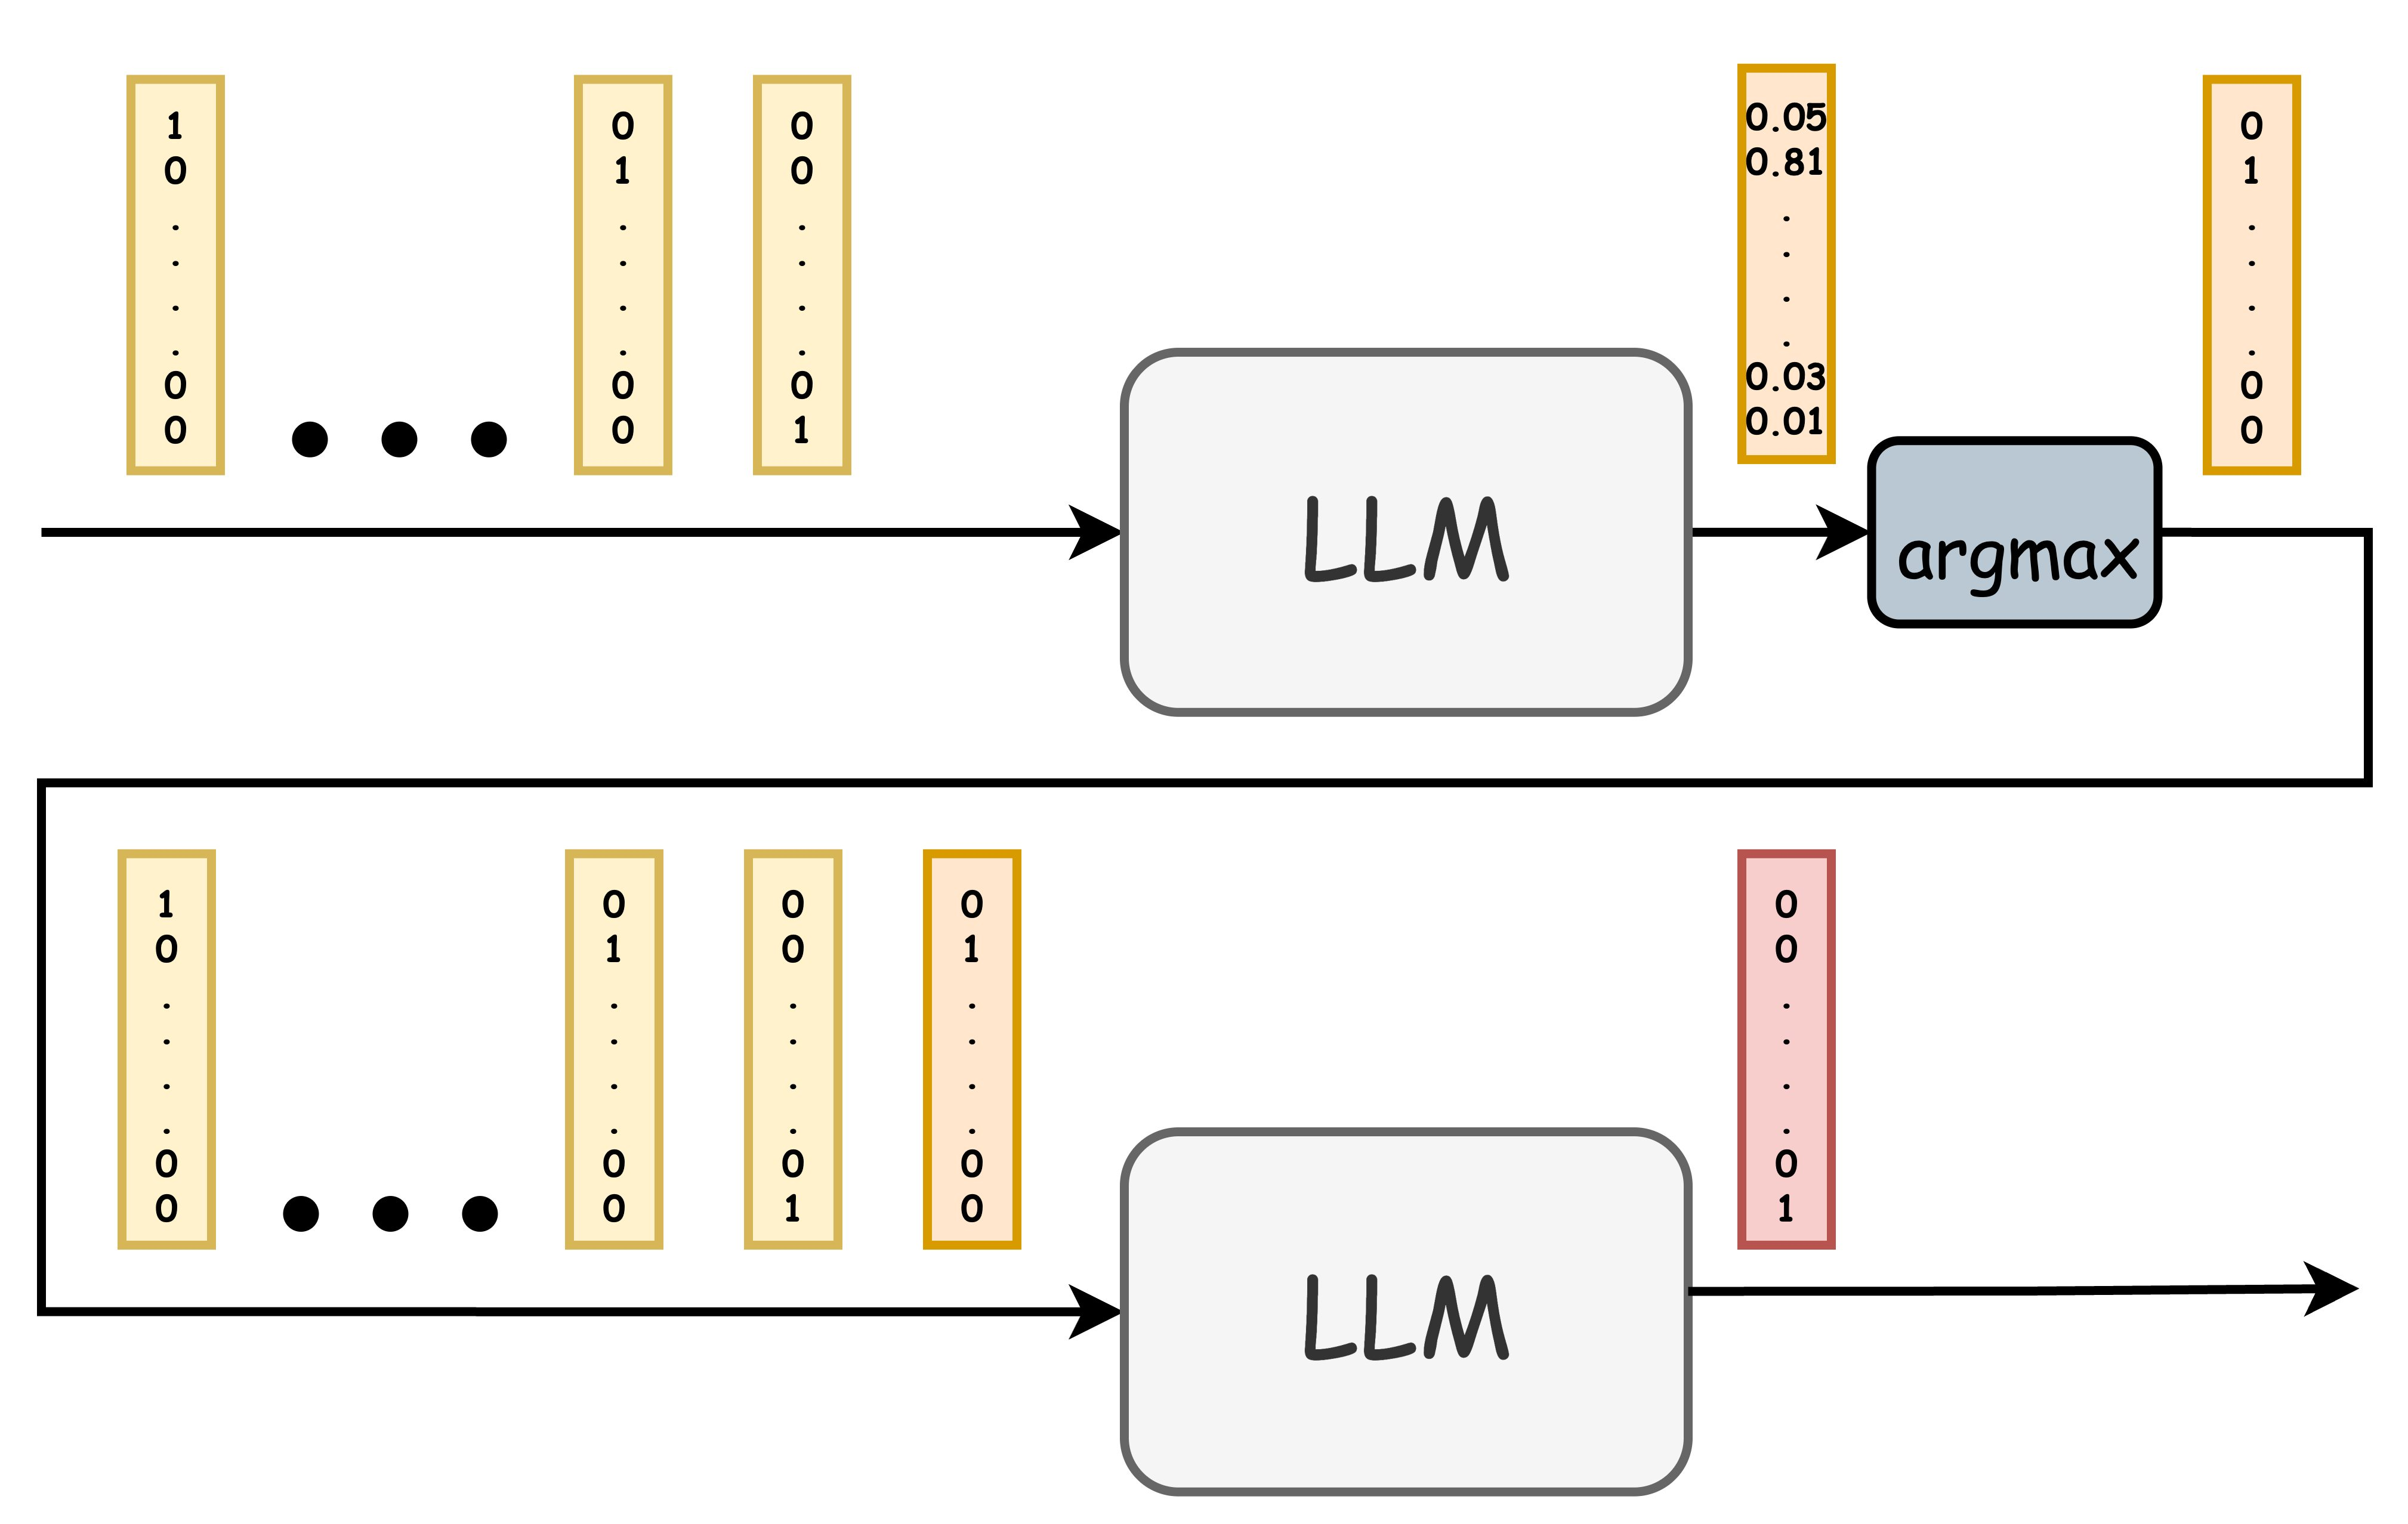
\includegraphics[width=0.5\textwidth]{graphs/ser1.jpeg}
  \caption{Visualization of the "without training" approach, p1}
  \label{fig:ser1}
\end{figure}

\begin{figure}[hbt]
  \centering
  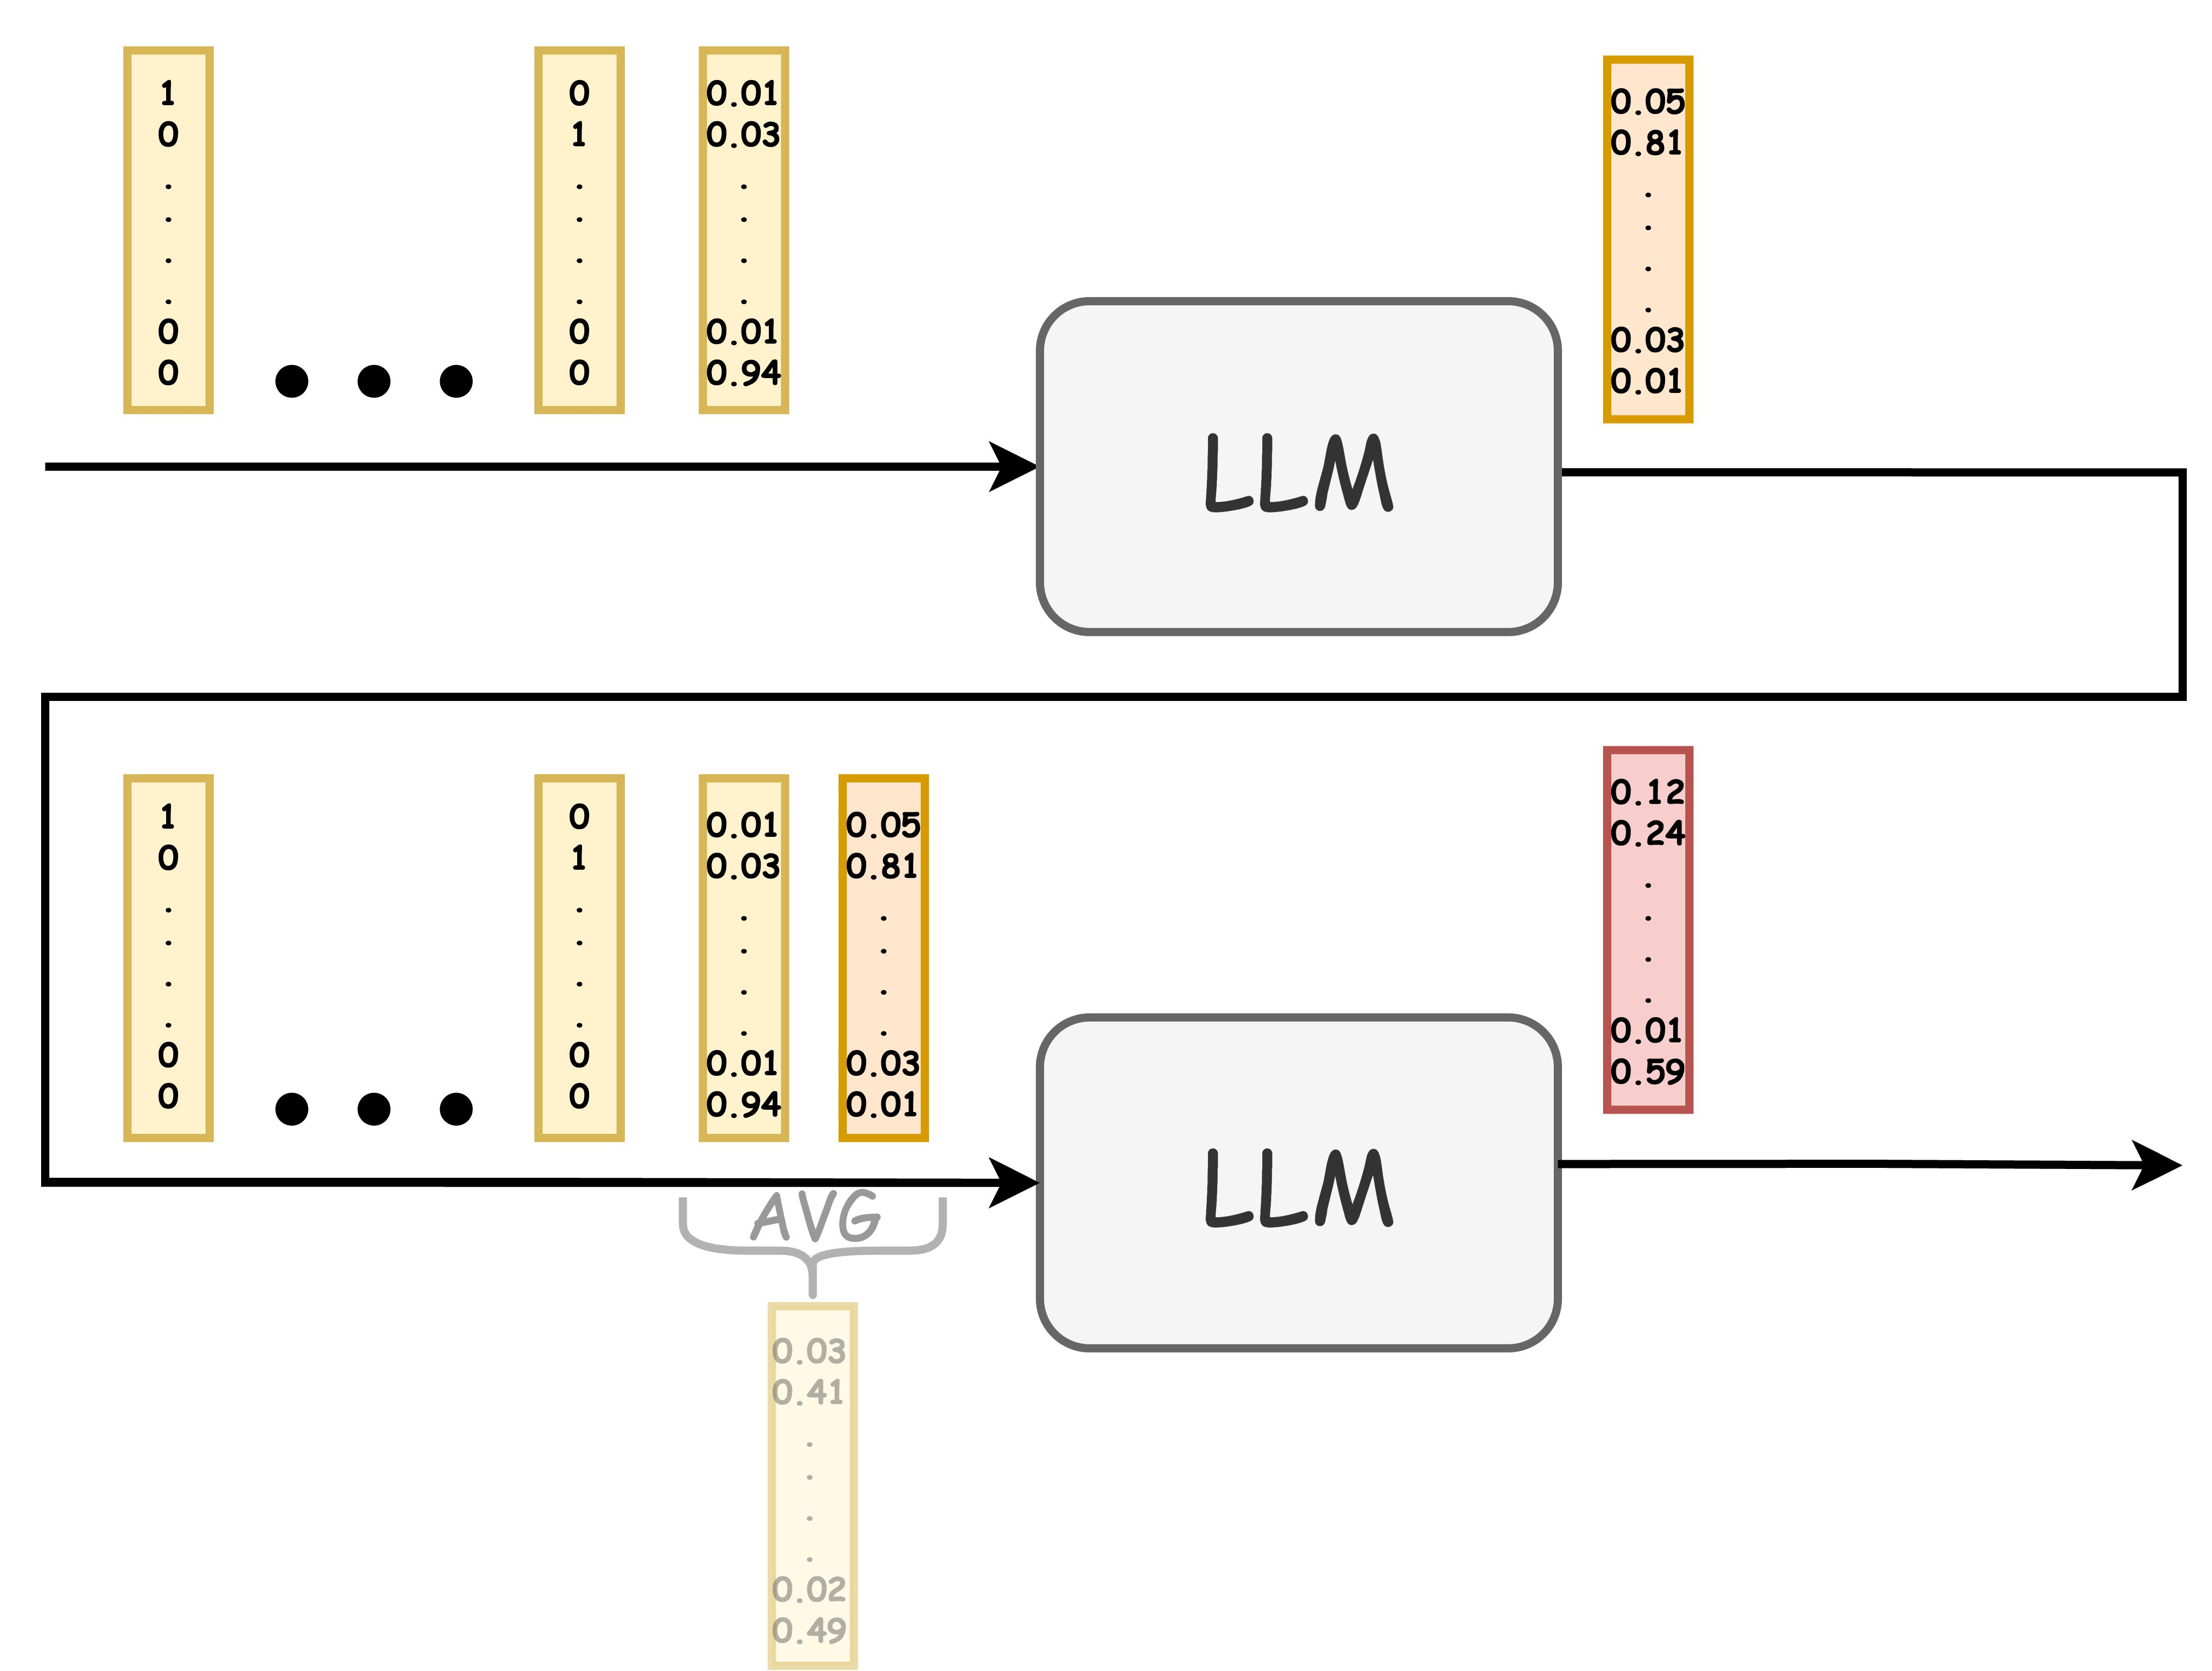
\includegraphics[width=0.3\textwidth]{graphs/ser2.jpeg}
  \caption{Visualization of the "without training" approach, p2}
  \label{fig:ser2}
\end{figure}


\section{Initial Prototype Experiments: First Attempts at Training}

Having established in \S5.1 that naively averaging ("avg, ×2") adjacent embeddings sharply degrades QA quality, we next asked whether a learned projection inserted at the embedding interface could recover performance under the same $2\times$ compression ratio.
The motivation was that, if the embedding manifold is non-linear, a trained projection might learn a geometry-preserving down-map that simple averaging cannot provide.
The baseline (Step 1) and the "soft/hard mix works" observation (Step 2) are illustrated in \ref{fig:steps1-3} and frame this question empirically.

\begin{figure}[hbt]
  \centering
  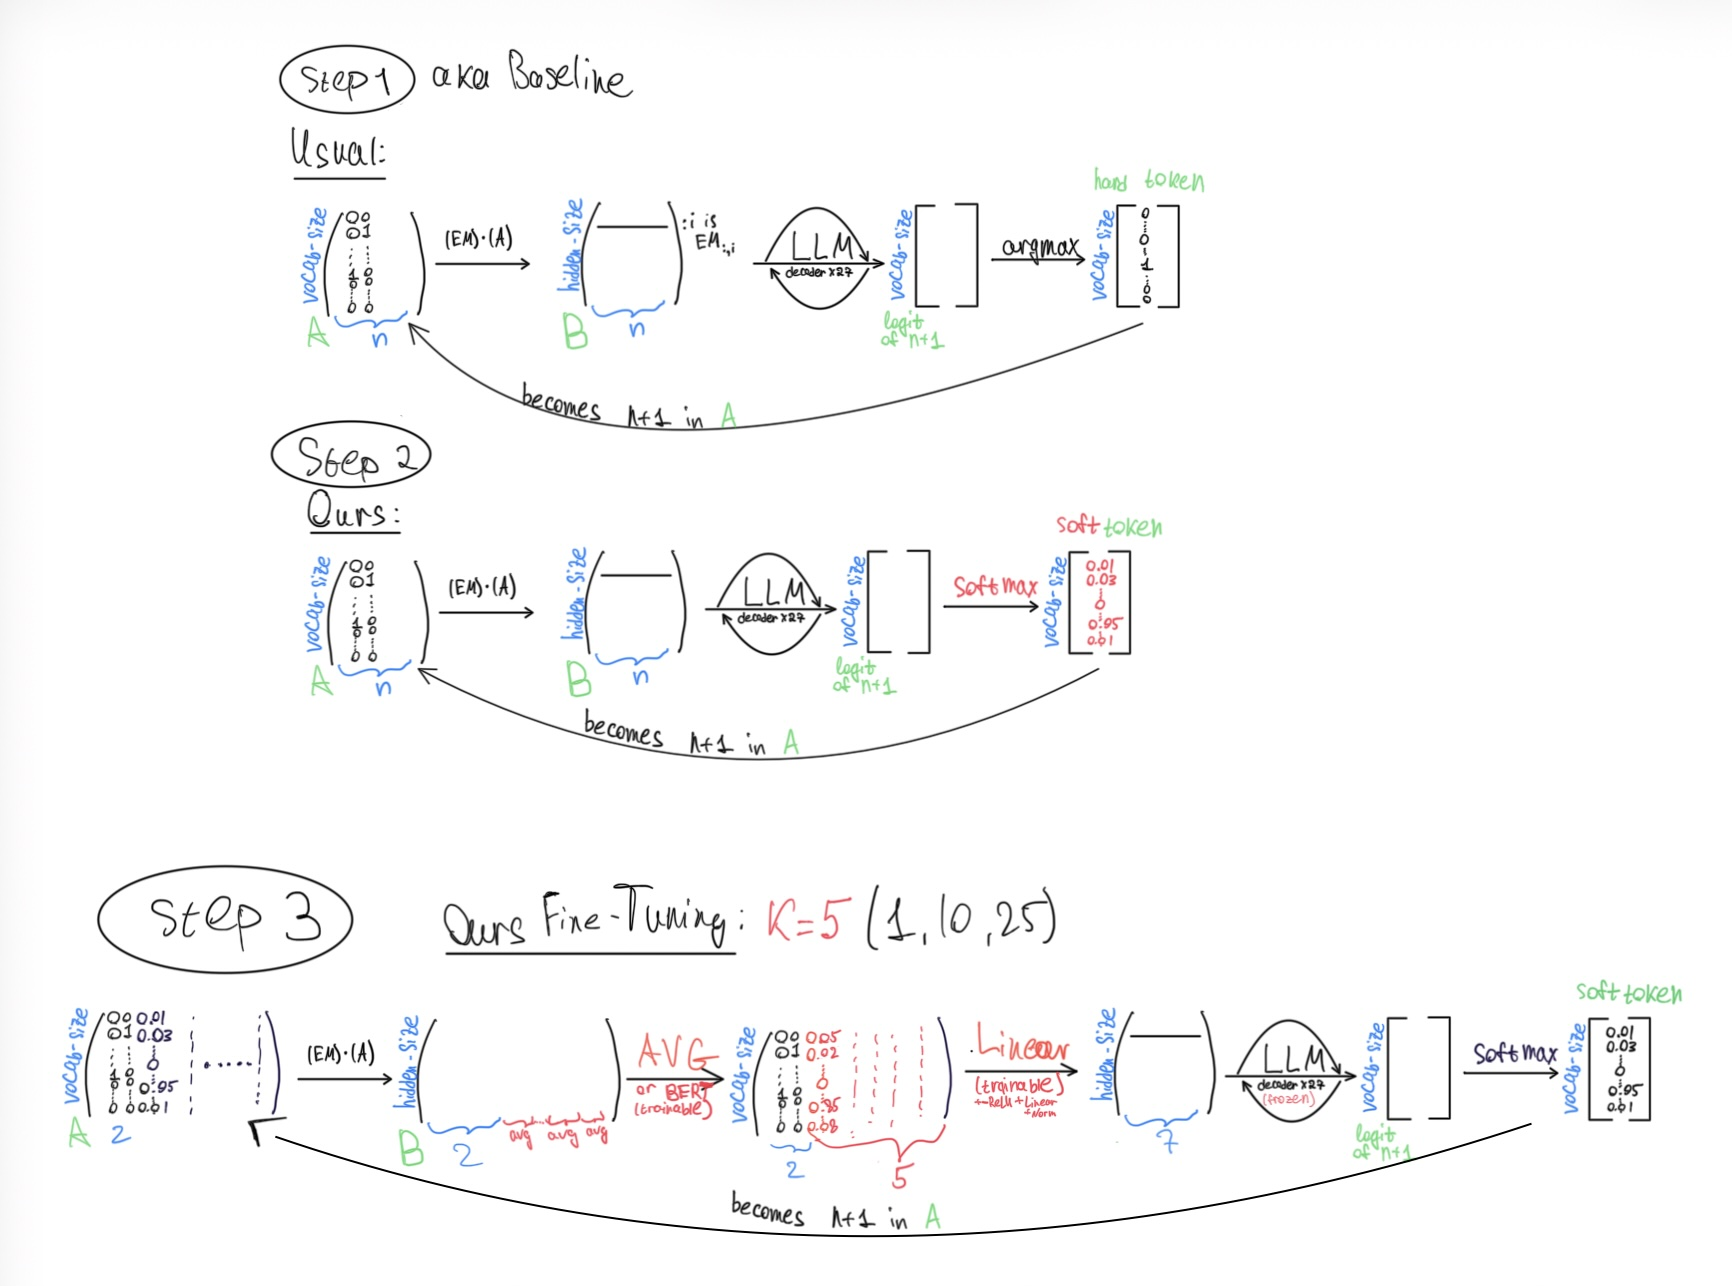
\includegraphics[width=0.5\textwidth]{graphs/steps1-3.jpg}
  \caption{Visualization of the baseline approach, step 1-3}
  \label{fig:steps1-3}
\end{figure}  

\paragraph{Architectural variants}
We explored minimal-capacity projections that compress two adjacent hidden vectors into one "soft token" acceptable to the frozen decoder.
The first family was a \textbf{linear projector}, $g_\theta:\mathbb{R}^{2d}\to\mathbb{R}^{d}$, applied to $[e_{2t-1};e_{2t}]$ with optional residual gating on the arithmetic mean to stabilize scale.
The second family was a shallow non-linear MLP (one--two layers with GELU), again mapping $2d\to d$.
A third variant inserted a full BERT encoder \cite{devlin2018bert} (12 layers, 768-dimensional hidden states) to process the concatenated embeddings $[e_{2t-1};e_{2t}]$ and produce a single compressed representation, which was then projected back to the decoder's dimensionality.
This encoder-based approach provided substantially higher capacity than the shallow projections, allowing the model to learn more complex compression patterns through its multi-layer self-attention mechanism.
These designs follow the "trainable averaging" schematics shown on \ref{fig:step35}.

\begin{figure}[hbt]
  \centering
  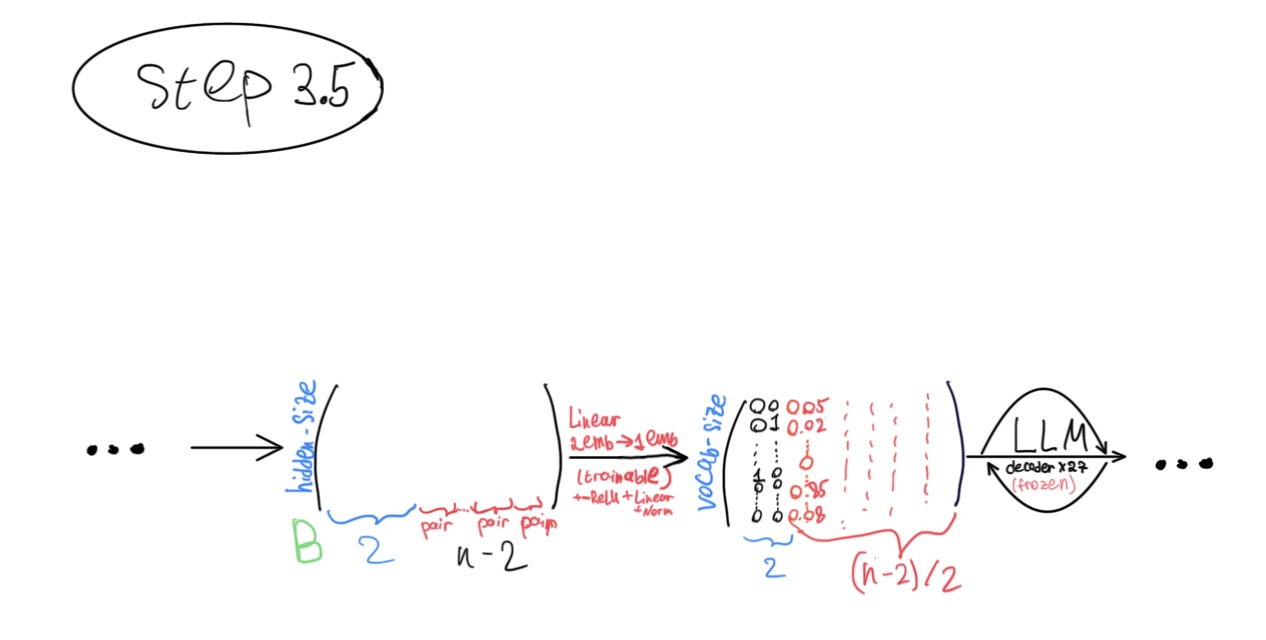
\includegraphics[width=0.5\textwidth]{graphs/step3.5.jpg}
  \caption{Visualization of the experimental setup, step 3-5}
  \label{fig:step35}
\end{figure}  

\paragraph{Training protocol and results}
All experiments used the SQuAD \cite{squad} "context-embed" setting from \S5.1, keeping Qwen3-8B frozen and training only the projection parameters via token-level cross-entropy on answer continuations.
After verifying the pipeline on a single batch, we trained on SQuAD train and evaluated on validation.
Across linear, MLP, and BERT projections, models quickly overfit but did not generalize: validation loss flattened after early improvement (\ref{fig:losses_squad_1}), and EM/F1 remained well below the hard-token baseline, never closing the large gap to the no-compression control (e.g., the $\sim 50\%$--$80\%$ relative F1 drop visible for averaging).

\begin{figure}[hbt]
  \centering
  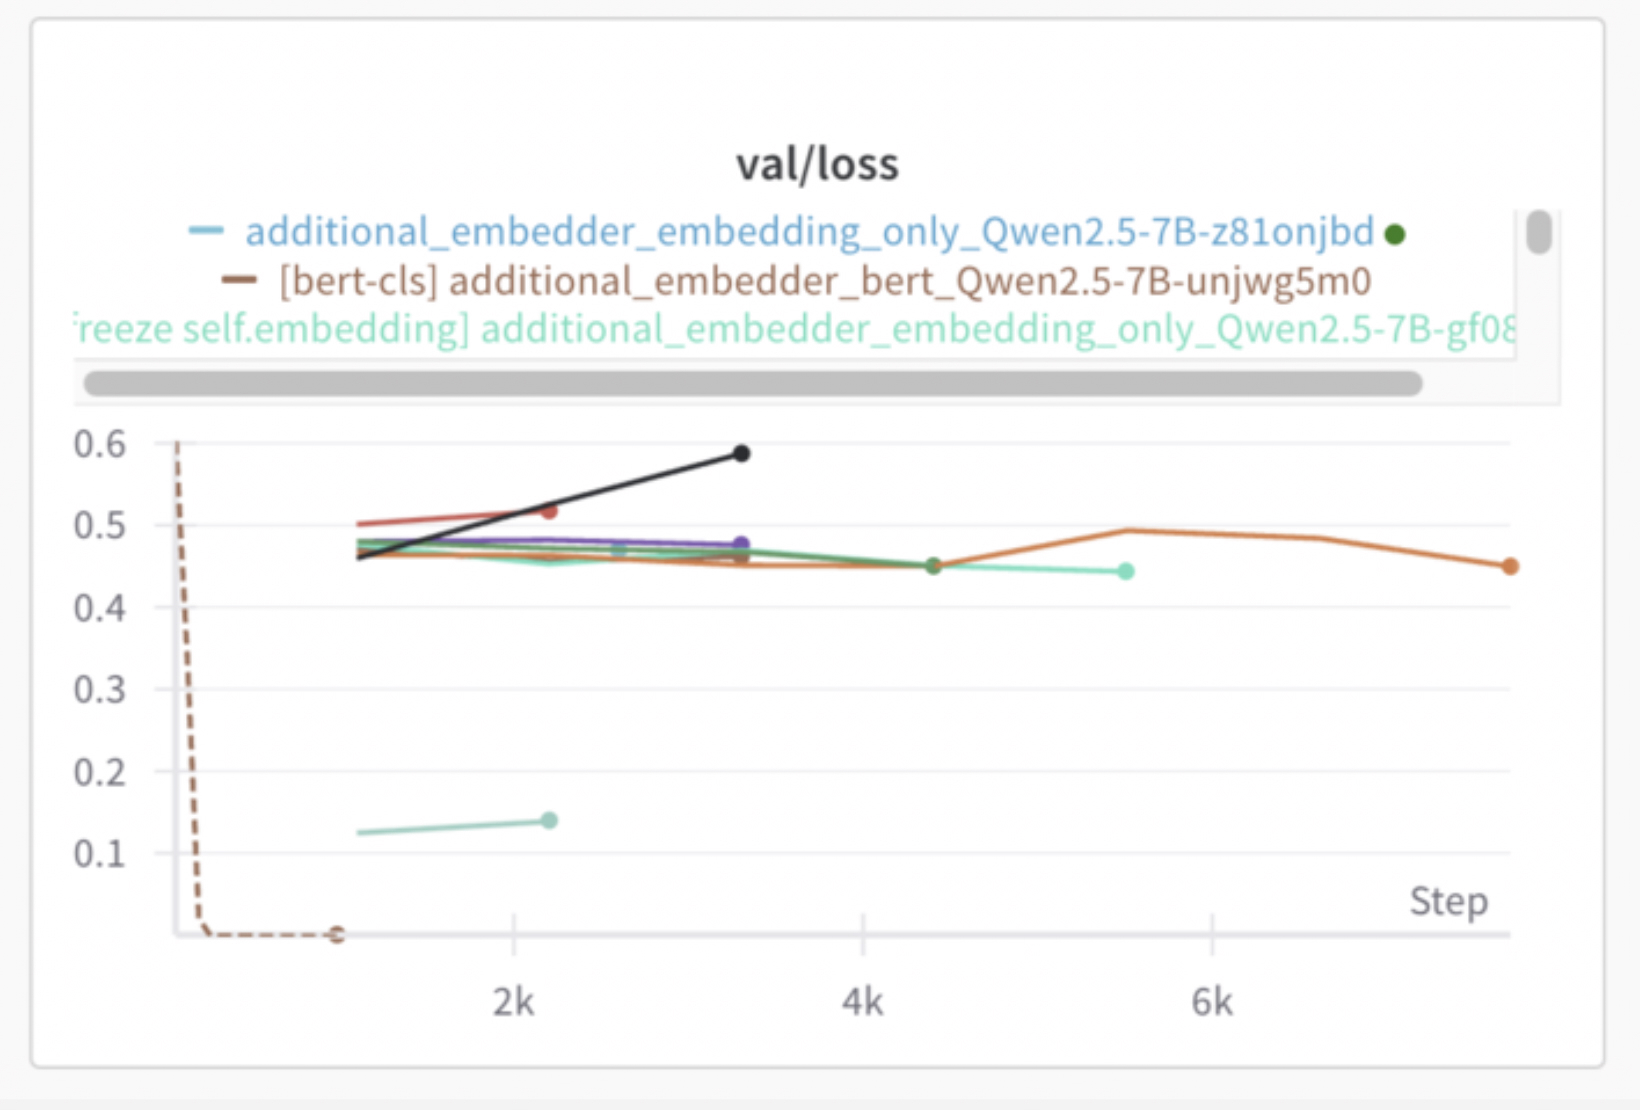
\includegraphics[width=0.5\textwidth]{graphs/losses_squad_1.jpg}
  \caption{Validation loss curves for the SQuAD generalization experiment using linear, MLP and BERT}
  \label{fig:losses_squad_1}
\end{figure}  


\paragraph{Ablation studies}
We varied:
\begin{itemize}
    \item projection type (linear vs.\ 1- or 2-layer MLP),
    \item normalization (pre/post LayerNorm, scale-preserving residual gates),
    \item regularization (weight decay, dropout), and
    \item the decision to re-project via vocabulary space versus staying in hidden space.
\end{itemize}
We also tried unfreezing the token embedding table while keeping the transformer blocks frozen.
None of these changes altered the qualitative outcome: projections still overfit quickly and failed to surpass the baseline (\ref{fig:steps1-3}) in EM/F1.
These negative findings echo the summary on the checkpoint deck ("all our fine-tuning techniques do not recover quality").

\paragraph{Hypotheses for the failure}
Two factors appear decisive.

Firstly, we hypothesize that if the embedding manifold is not smooth, merging two embeddings into one may lose critical geometric structure that the frozen decoder relies on, making it impossible for a simple projection to preserve the information needed for downstream tasks.


Secondly, we hypothesize that the fundamental limitation is the expressive power of the overall model architecture.
Even though the BERT encoder contains 0.1B parameters (more than the projections), it lacks the capacity to learn effective compression when paired with a frozen 8B decoder.

This observation motivated our transition to the ICAE framework, where training LoRA adapters ($\approx$2\% of the 8B model's weights) provides substantially greater expressive power by modulating the decoder's internal representations, despite involving fewer trainable parameters than the full BERT encoder.


\paragraph{Summary}
The experiments illustrated in \ref{fig:step35} demonstrate that trainable projections are insufficient to recover QA performance under $\approx2\times$ compression.
These results motivated us to explore larger-scale training approaches and alternative solutions such as the ICAE framework.


\textbf{TODO: I STOPPED HERE}

% ========================================
% SECTION 5.2: EVALUATION ON GENERAL TEXT RECONSTRUCTION
% ========================================
\section{ICAE Pretraining and Evaluation on General Text Reconstruction}

Pretrained ICAE \cite{ge_-context_2024} demonstrated the ability to decompress general texts almost perfectly.
High BLEU scores were achieved on datasets like PWC (99.1 for Mistral-7B, 99.5 for Llama-2-7B) and SQuAD (98.1 for Qwen3-8B), indicating that memory slots retained almost all context information for contexts up to 400 tokens.
Analysis of reconstruction errors showed patterns similar to human memorization mistakes (e.g., restoring "large pretrained language model" as "large pretrained model"), suggesting the model selectively emphasizes or neglects information based on its understanding.


% ========================================
% SECTION 5.3: EVALUATION ON QUESTION ANSWERING TASKS (OFFLINE)
% ========================================
\section{ICAE Fine-Tuning and Evaluation on Question Answering Tasks}

When fine-tuned on QA tasks (SQuAD), ICAE-FT \cite{ge_-context_2024} achieved high F1 (73) and Exact Match (69\%) scores, performing well compared to LoRA-FT baselines.
The quality of the compressed representation was shown to significantly outperform summaries generated by GPT-4 under the same length constraint (128 tokens).

\begin{table}[h]
    \centering
    \begin{tabular}{lccc}
        \toprule
        \textbf{Model} &
        \textbf{Compression} &
        \textbf{Exact Match} &
        \textbf{F1} \\
        \midrule
        Mistral-7B (no FT)          & ×$1$         & 49 & 68 \\
        LoRA-FT baseline            & ×$1$         & \underline{59} & \underline{65} \\
        ICAE FT (PwC, authors)       & ×$1.7\pm0.7$ & 41 & 57 \\
        ICAE FT (SQuAD, ours)              & ×$1.7\pm0.7$ & \textbf{69} & \textbf{73} \\
        \bottomrule
    \end{tabular}
    \caption{ICAE averaging on SQuAD}
    \label{tab:icae_squad}
\end{table}


% ========================================
% SECTION 5.4: EVALUATION ON AGENTIC PERFORMANCE (SWE-BENCH)
% ========================================
\section{ICAE Fine-Tuning and Evaluation on SWE-bench Verified}

% ========================================
% SECTION 5.x: DISABLING THINKING EXPERIMENTS
% ========================================
\section{Disabling Thinking Experiments}
\label{sec:disabling_thinking}

We evaluated the impact of disabling thinking by inserting the token sequence \texttt{\textbackslash think \textbackslash think} with a newline marker during decoding.
We tested two variants: adding the sequence after every step and adding it only once at the end.
Surprisingly, the approach commonly suggested by authors (frequent insertion) yielded worse output quality than the minimal, end-only variant in our setting.
We note that related observations of atypical Qwen3 behavior under prompting heuristics have been reported anecdotally; a systematic investigation is out of scope for this work. (as a result e.g. coder-30bA3 has no thinking mode at all)
Further details and ablations are left for future work.

Efficiency Results: ICAE \cite{ge_-context_2024} compression led to measurable efficiency improvements, achieving a theoretically 10\% faster mean tool-call generation time than the vanilla baseline (e.g., 0.4880s vs 0.5437s).
Furthermore, latency tests showed speedups of 2.2× to 3.6× in total time for inference.
Token-wise Accuracy vs. Resolved Rate: Although token-wise accuracy performed on par with (or slightly better than) the vanilla Qwen baseline (e.g., 0.9089 vs 0.9000), this metric was noted to be problematic ("token-wise accuracy is bullshit") and decoupled from true task success.
End-to-End Task Success: The primary negative finding was that the model with compression resolved significantly fewer than 50\% as many issues as the original Qwen model on the SWE-bench Verified dataset.

\begin{table}[h]
    \centering
    \setlength{\tabcolsep}{6pt}
    \begin{tabular}{llcc}
        \toprule
        \textbf{Encoder} & \textbf{Decoder} & \textbf{Accuracy} & \textbf{Mean tool-call time (s)} \\
        \midrule
        % --- Baseline encoder
        —                        & Full-FT   & 0.9484 & 1.24 \\
        —                        & LoRA-FT   & 0.9118 & 1.24 \\
        —                        & Qwen           & 0.8967 & 1.23 \\
        \addlinespace
        % --- Ablations
        del long obs-s             & Qwen           & 0.8873 & 0.44 \\
        del all obs-s              & Qwen           & 0.8802 & 0.39 \\
        \addlinespace
        % --- ICAE (Qwen pretrained) encoder
        ICAE (LoRA-PT w/ Full-FT)   & Full-FT   &  0.9219    &  — \\
        ICAE (LoRA-PT w/ Qwen)    & Qwen           &  0.8808 & \textbf{1.12 (0.31+0.81)} \\
        \addlinespace
        % --- ICAE (Qwen-LoRA-FT) encoder
        ICAE (LoRA-FT)         & Full-FT   &  ?   & —  \\
        ICAE (LoRA-FT)         & LoRA-FT   & 0.9263   & —  \\
        ICAE (LoRA-FT)         & Qwen           & 0.9020 & — \\
        % bad-seed ICAE (LoRA-FT)         & Qwen           & 0.8918 & — \\       

        
        \bottomrule
    \end{tabular}
    \caption{No think bug table. Qwen and ICAE future variants. FT=FineTuning, PT=PreTraining}
    \label{tab:icae_variants}
\end{table}

\begin{table}[h]
    \centering
    \small
    \setlength{\tabcolsep}{4pt}
    % --- Добавлены рамки по краям таблицы для цельного вида ---
    \begin{tabular}{|ll|ccc|}
        \hline
        \textbf{Encoder} & \textbf{Decoder} & \textbf{Acc.} & \textbf{Time (s)} & \textbf{Resolved (/500)} \\
        \hline
        % --- Baseline encoder
        —                         & Qwen-Full-FT   & 0.9484 & 1.24                      & —         \\
        —                         & Qwen-LoRA-FT   & 0.9118 & 1.24                      & 10        \\
        —                         & Qwen           & 0.8967 & 1.23                      & 26        \\
        \hline
        % --- ICAE (Qwen-LoRA-FT) encoder
        ICAE (Qwen-LoRA-FT)       & Qwen           & 0.9020 & —                         & 11        \\
        ICAE (Qwen-LoRA-FT)       & Qwen-LoRA-FT   & 0.9263 & —                         & 3 (overfit?) \\
        ICAE (Qwen-LoRA-FT)       & Qwen-Full-FT   & ?      & —                         & —         \\
        \hline
        % --- Ablations
        del long obs-s            & Qwen           & 0.8873 & 0.44                      & 1         \\
        del all obs-s             & Qwen           & 0.8802 & 0.39                      & 0         \\
        \hline
        % --- ICAE (Qwen pretrained) encoder
        ICAE (Qwen-LoRA-PT w/ Q-Full-FT) & Qwen-Full-FT   & 0.9219 & —                         & —         \\
        ICAE (Qwen-LoRA-PT w/ Qwen)      & Qwen           & 0.8808 & \textbf{1.12 (0.31+0.81)} & —         \\
        \hline
    \end{tabular}
    \caption{No think bug table. Qwen and ICAE future variants. FT=FineTuning, PT=PreTraining}
    \label{tab:qwen_icae_variants_absolute}
\end{table}

\begin{figure}[hbt]
  \centering
  
\includegraphics[width=0.8\textwidth]{graphs/mega-1.jpeg}
  \caption{ICAE application to SWE-bench - Results 1}
  \label{fig:mega1}
\end{figure}

\begin{figure}[hbt]
  \centering
  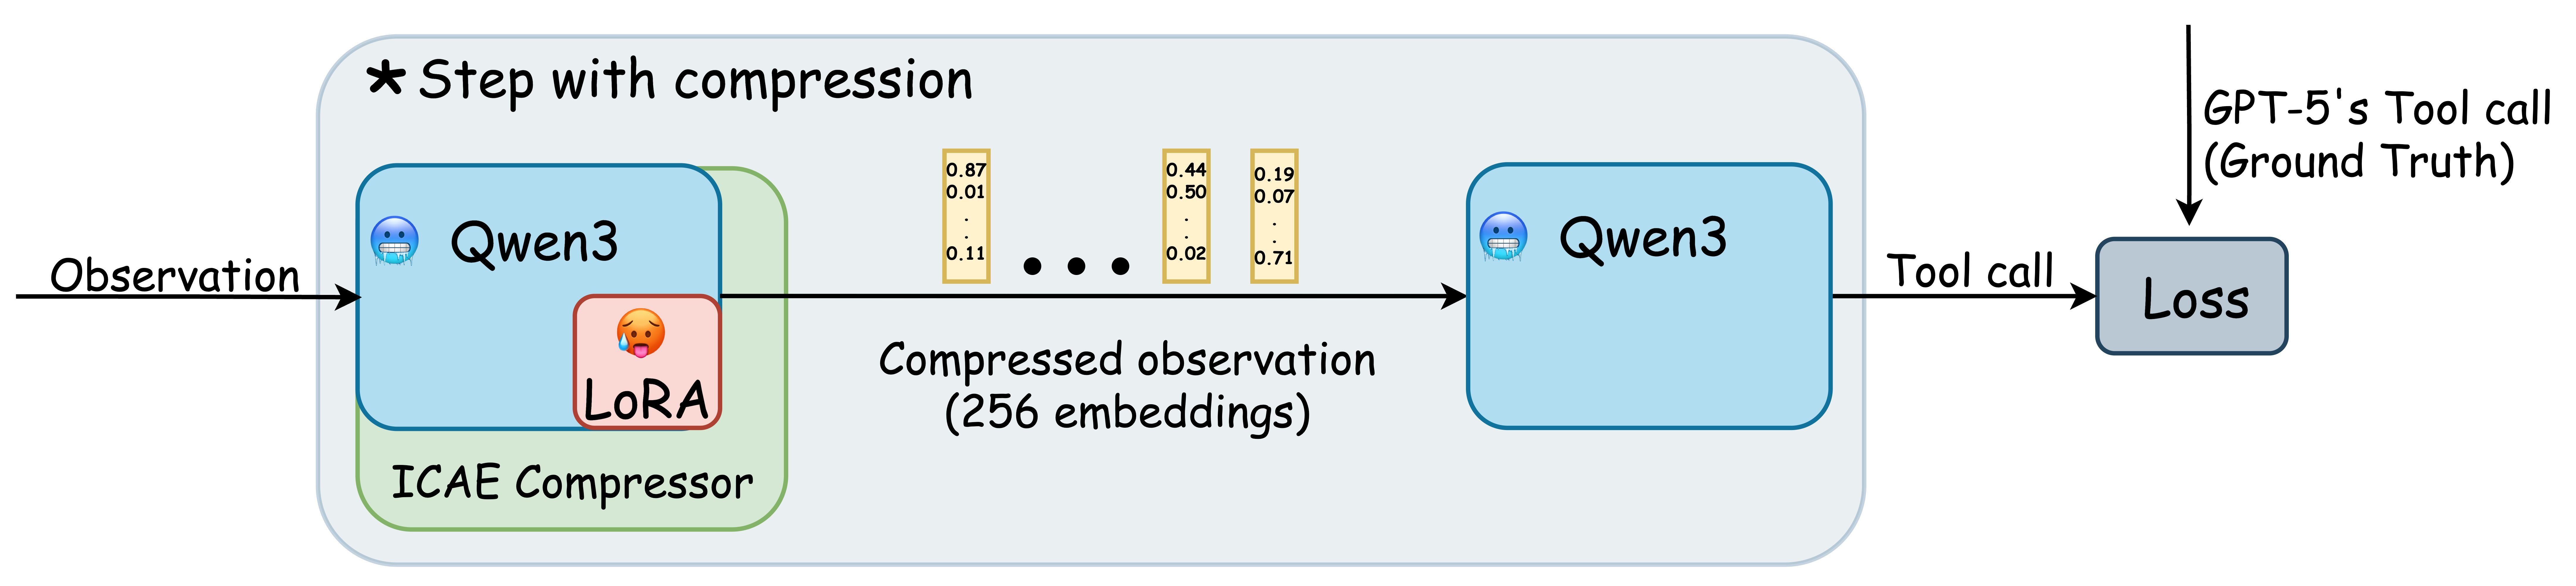
\includegraphics[width=0.8\textwidth]{graphs/mega-2.jpeg}
  \caption{ICAE application to SWE-bench - Results 2}
  \label{fig:mega2}
\end{figure}


% ========================================
% SECTION 5.5: DISCUSSION OF AGENTIC FAILURE HYPOTHESES
% ========================================
\section{Discussion of Agentic Failure Hypotheses}

Hypotheses for the end-to-end performance degradation include Representation–behavior mismatch, where the compression perturbs the decoder's behavior necessary for tool use.
Other factors include reconstruction quality falloff for specialized content like code files, and potential overfitting to labels demonstrated by high local accuracy but low resolved rates.
